% !TEX root = ../main.tex

% 分析与讨论	
\begin{table}
	\renewcommand\arraystretch{1.7}
	\begin{tabularx}{\textwidth}{|X|X|X|X|}
		\hline
		Major:& Physics &Grade:& 2022\\
		\hline
		Name: & 杨舒云 \& 戴鹏辉 & Student number:& 22344020 \& 22344016\\
		\hline
		Date:& 2024/9/25 & Score: &\\
		\hline
	\end{tabularx}
\end{table}
\section{ET2-1 Welding and Debugging of Bluetooth Speakers \\ Analysis \& Discussion}


%---------------------------------------------------------------------
% 数据处理
\subsection{Data Processing}

% 分析
\subsubsection{Analysis}
In this part, we will solve the requested problems .
\begin{enumerate}
	\item Analyze the function of the circled circuit in \cref{fig:question}.
	
	\begin{figure}[htbp]
		\centering
		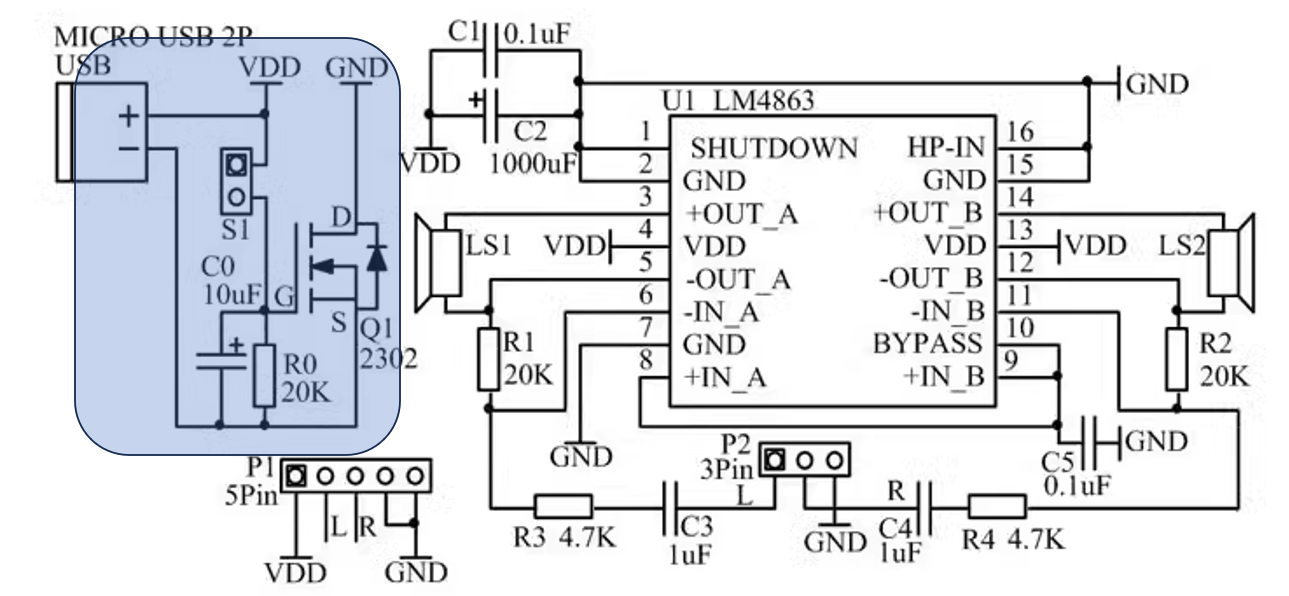
\includegraphics[width=0.7\textwidth]{ET2_1_question.png}
		\caption{The circled circuit}
		\label{fig:question}
	\end{figure}
	
	The circuit is powered through a USB cable, where Q1, R0, S1, and C0 form an electronic switch to replace a common mechanical switch. S1 is a mercury switch, which relies on the flow of mercury to establish or break the connection. When the speaker is placed upright, the mercury switch conducts. If the speaker is tilted, the mercury switch breaks. This principle is used to control the on-off state of the circuit. Q1 is an N-channel MOSFET, which requires a positive voltage at its gate to conduct. When the mercury switch is on, the gate receives positive voltage, and Q1 conducts, providing power to the amplifier circuit. When the mercury switch is off, the gate is grounded through resistor R0, causing Q1 to turn off, thereby cutting off power to the amplifier circuit. Capacitor Co is used for switch debounce. Additionally, the operating current of the mercury switch is small; a 3 mm mercury switch cannot handle more than 300 mA of current. The speaker, however, requires approximately 1 A of operating current, hence a MOSFET is needed for control.
	
	More information:
	\begin{itemize}
		\item MOSFET(Metal-Oxide-Semiconductor Field-Effect Transistor)是一种场效应晶体管,通常用于开关和放大应用。它具有三个主要电极:栅极(Gate, G)、漏极(Drain, D)、源极(Source, S)。本电路中使用的是P沟道MOSFET(型号为2302),它的工作原理是当栅极电压比源极电压更低时,MOSFET导通,从源极到漏极的电流被允许通过;而当栅极电压和源极电压相等或栅极电压比源极电压高时,MOSFET关闭,从而阻止电流流动。
		
		\item 在电路中,电源通过Micro USB接口输入,并提供VDD电压。电容C0(10μF)作为旁路电容,用于滤波,降低电源电压中的噪声,提供稳定的直流电压给后续电路。PMOS管Q1(型号为2302)是整个电路的核心开关元件,它与机械开关S1一起用于控制电源是否为后续电路供电。当S1闭合时,栅极通过电阻R0(20kΩ)接地,形成一个负栅源电压,使Q1导通,从而使VDD电压能够传递给其他部分的电路;而当S1断开时,栅极通过R0与源极电压趋于同电位(无负压),使Q1截止,切断电源。电阻R0的作用是在开关S1打开时,将Q1的栅极电压拉高至接近源极电压(即VDD),使得Q1能够正确关闭。当S1闭合时,R0限制了从栅极到地的电流,确保栅极电压足够低于源极,使Q1导通。另外,PMOS管Q1内部还自带有一个体二极管(图中箭头所示),它用于防止外部电压反向输入。如果电源方向接反,该二极管会阻断反向电流,防止损坏电路的其他元件。
		
		\item 这个电路的整体工作流程是:当插入电源时,输入电压经过C0滤波以确保其平稳;然后通过S1控制是否将电压VDD传递到下游电路。当S1闭合时,Q1导通,电源得以供给后续电路;当S1断开时,Q1截止,电源被切断,防止任何电流流动。这样设计的电路在实际应用中非常广泛,例如用于便携式电子设备中,用户可以方便地通过机械开关来控制电路是否供电,同时也具备反向电流保护的功能,防止因误操作造成电路的损坏。
	\end{itemize}
	
	\item Analyze the voltage and power amplification of the LM4863 amplifier circuit.
	
	\begin{figure}[htbp]
		\centering
		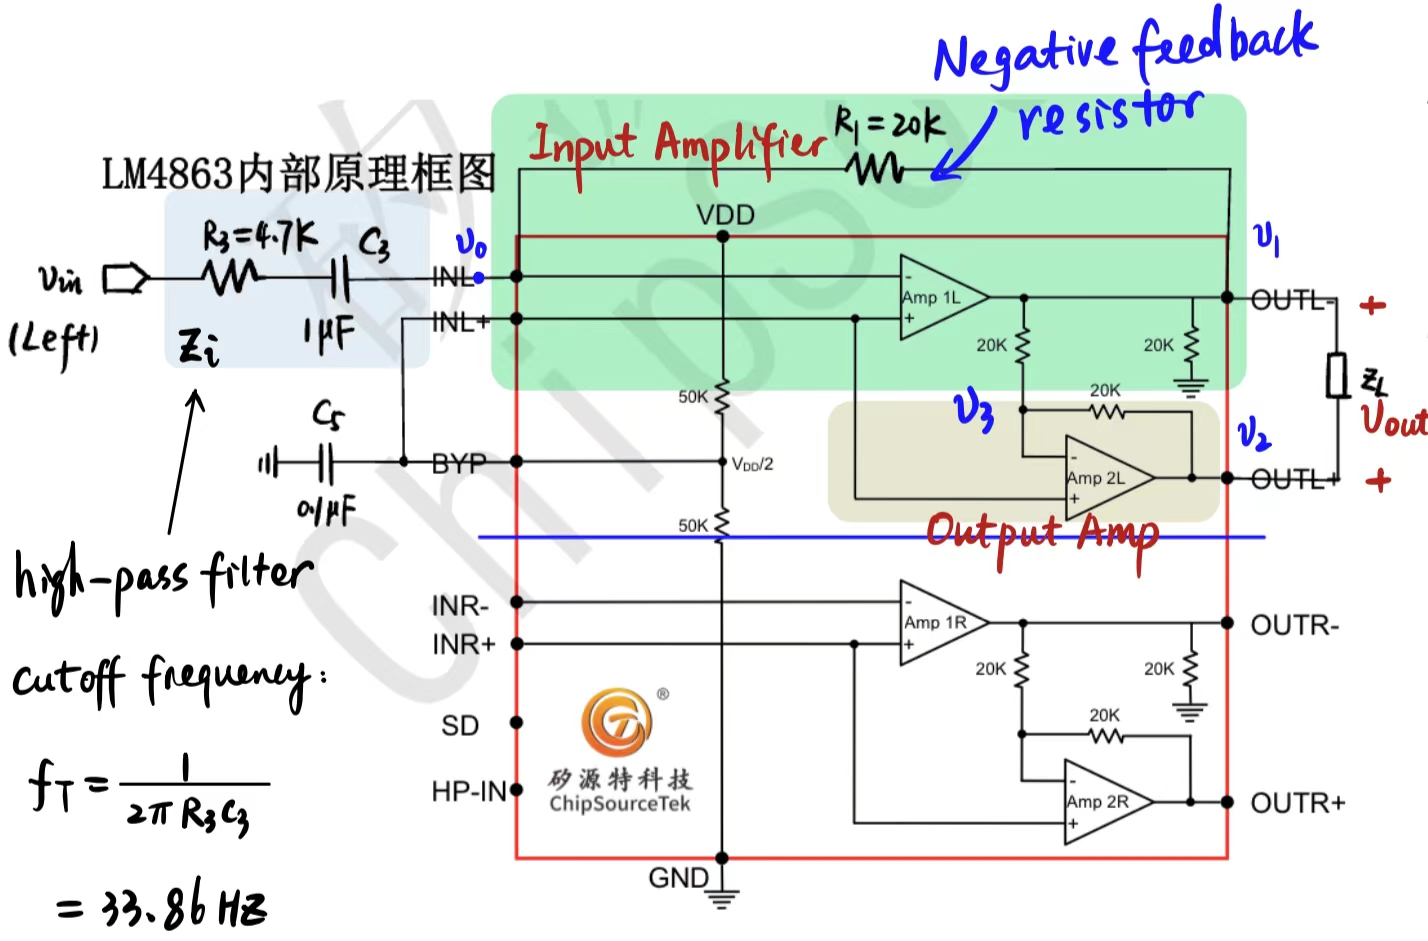
\includegraphics[width=0.7\textwidth]{ET2_1_analysis.jpg}
		\caption{The analysis of circuit}
		\label{fig:analysis}
	\end{figure}
	
	As we can see in \cref{fig:analysis}, it's exactly the same between the left tone and right tone. Thus, we just need to analyze the half.
	
	For Amp 1L, $v_0=0$, $v_1=-\frac{R_1}{Z_i}v_{in}$, and $\frac{v_1-v_3}{20k\Omega}=\frac{v_3-v_2}{20k\Omega}$, so that $v_3 = (v_1 + v_2) / 2$.
	
	As op amplifier, $v_3=0\Rightarrow v_2=-v_1=\frac{R_1}{Z_i}v_{in}\Rightarrow v_{out} = v_2 - v_1 = \frac{2R_1}{Z_i}v_{in}$.
	
	Thus, voltage gain $A_v$:
	
	\[
	A_v = \frac{v_{\text{out}}}{v_{\text{in}}} = \frac{2R_1}{Z_i} = \frac{2R_1}{R_3 + \frac{1}{j\omega C_3}} = \frac{2j\omega C_3 R_1}{1 + j\omega C_3 R_3}
	\]
	
	\[
	|A_v| = \frac{4 \pi f C_3 R_1}{\sqrt{1 + (2 \pi f C_3 R_3)^2}}, \quad \arg(A_v) = \frac{\pi}{2} - \arctan(2 \pi f C_3 R_3)
	\]
	
	Generally, we can regard $C_3$ only as a filter capacitor ($C_3 \to \infty$) and calculate:
	
	\[
	|A_v| = \frac{2R_1}{R_3} = 8.51, \quad |A_v|_{\text{dB}} = 20 \log \frac{R_1}{R_3} = 18.6 \, \text{dB}
	\]
	
	System cutoff frequency:
	
	\[
	\text{Assume } |A_v| = \frac{\sqrt{2}}{2} \cdot \frac{2R_1}{R_3} \Rightarrow f_L = \frac{1}{2 \pi C_3 R_3} = 33.86 \, \text{Hz}
	\]
	
	We can see that the cutoff frequency is determined by the input RC filter network. That's because $v_0$ is equal to zero in small signal circuit and input signal just generate and propagate circuit instead of voltage into the amplifier.
	
	\[
	P_{\text{out}} = \frac{V_{\text{out}}^2}{R_L}, \quad S_{\text{in}} = \dot{U} \dot{I}^* = v_{\text{in}} \left( v_{\text{in}}^* \cdot \frac{1}{R_3 + j \omega C_3} \right) = \frac{|v_{\text{in}}|^2}{R_3 + j \omega C_3},
	\]
	
	\[
	P_{\text{in}} = \text{Re}(S_{\text{in}}) = \frac{(2\pi f C_3)^2 R_3}{1 + (2\pi f C_3 R_3)^2} |v_{\text{in}}|^2
	\]
	
	\[
	\Rightarrow G_p = \frac{P_{\text{out}}}{P_{\text{in}}} = \frac{1 + (2\pi f C_3 R_3)^2}{(2\pi f C_3)^2 R_3 R_L} \frac{|V_{\text{out}}|^2}{|V_{\text{in}}|^2} \approx 17.0
	\]
	
	\[
	(G_p)_{\text{dB}} = 10 \log G_p = 12.3 \, \text{dB @ } 1 \, \text{kHz}
	\]
	
	The above analysis results can be plotted as shown in the \cref{fig:outcome1} and \cref{fig:outcome2}.
	
	\begin{figure}[htbp]
		\centering
		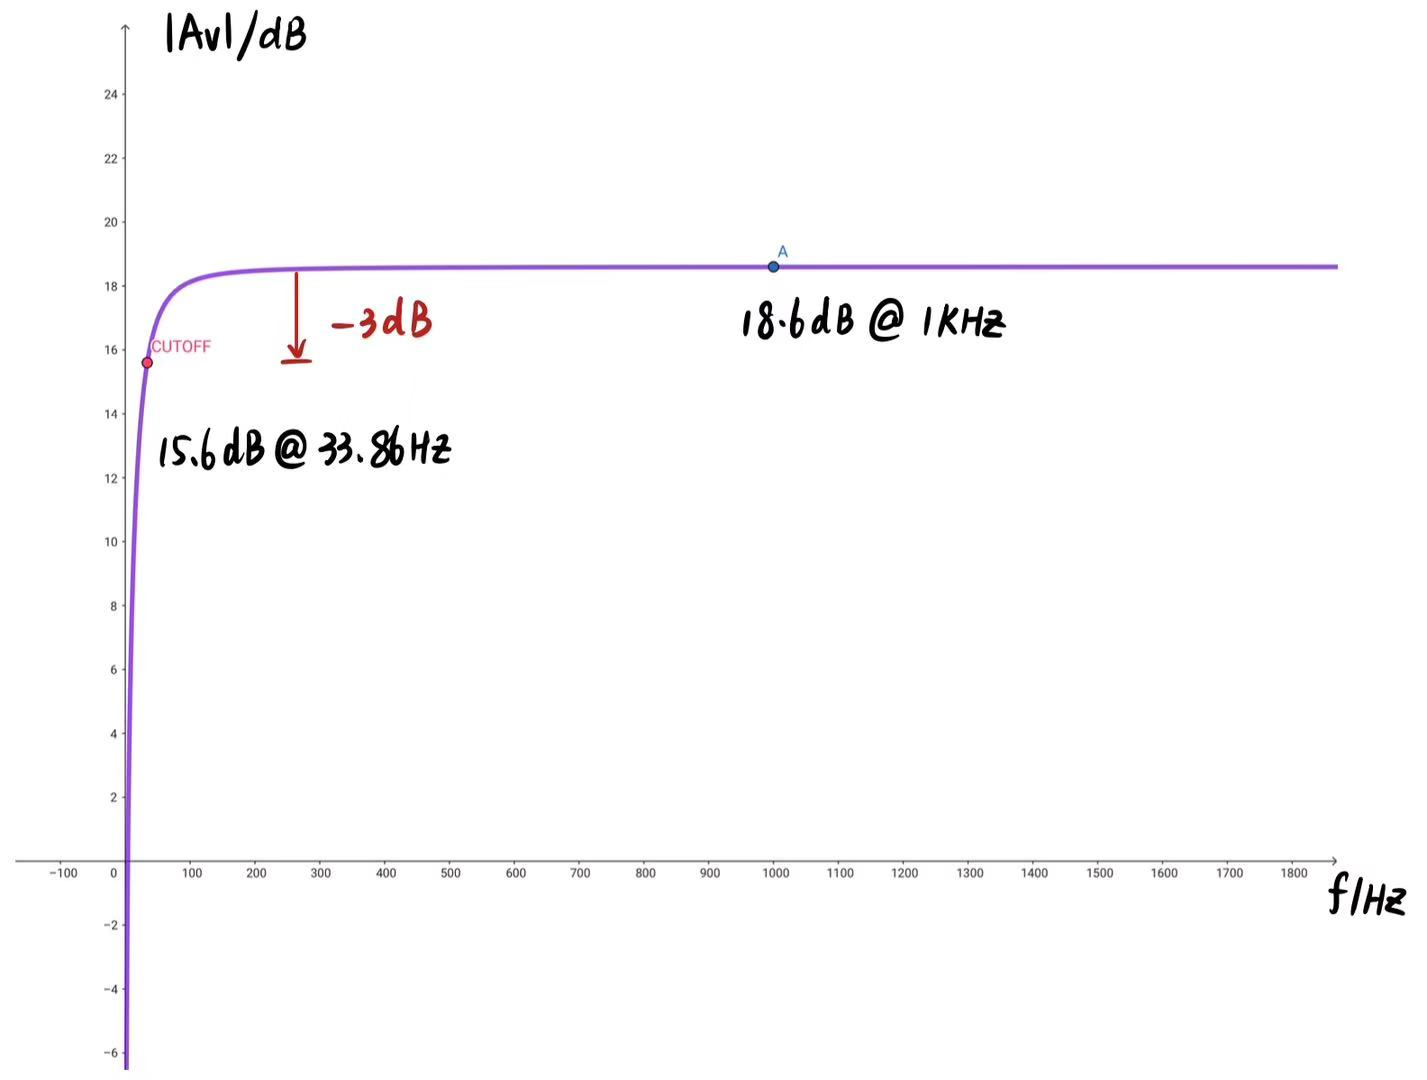
\includegraphics[width=0.7\textwidth]{ET2_1_analysis_outcome1.jpg}
		\caption{The analysis outcome of circuit ($A_v$-f)}
		\label{fig:outcome1}
	\end{figure}
	
	\begin{figure}[htbp]
		\centering
		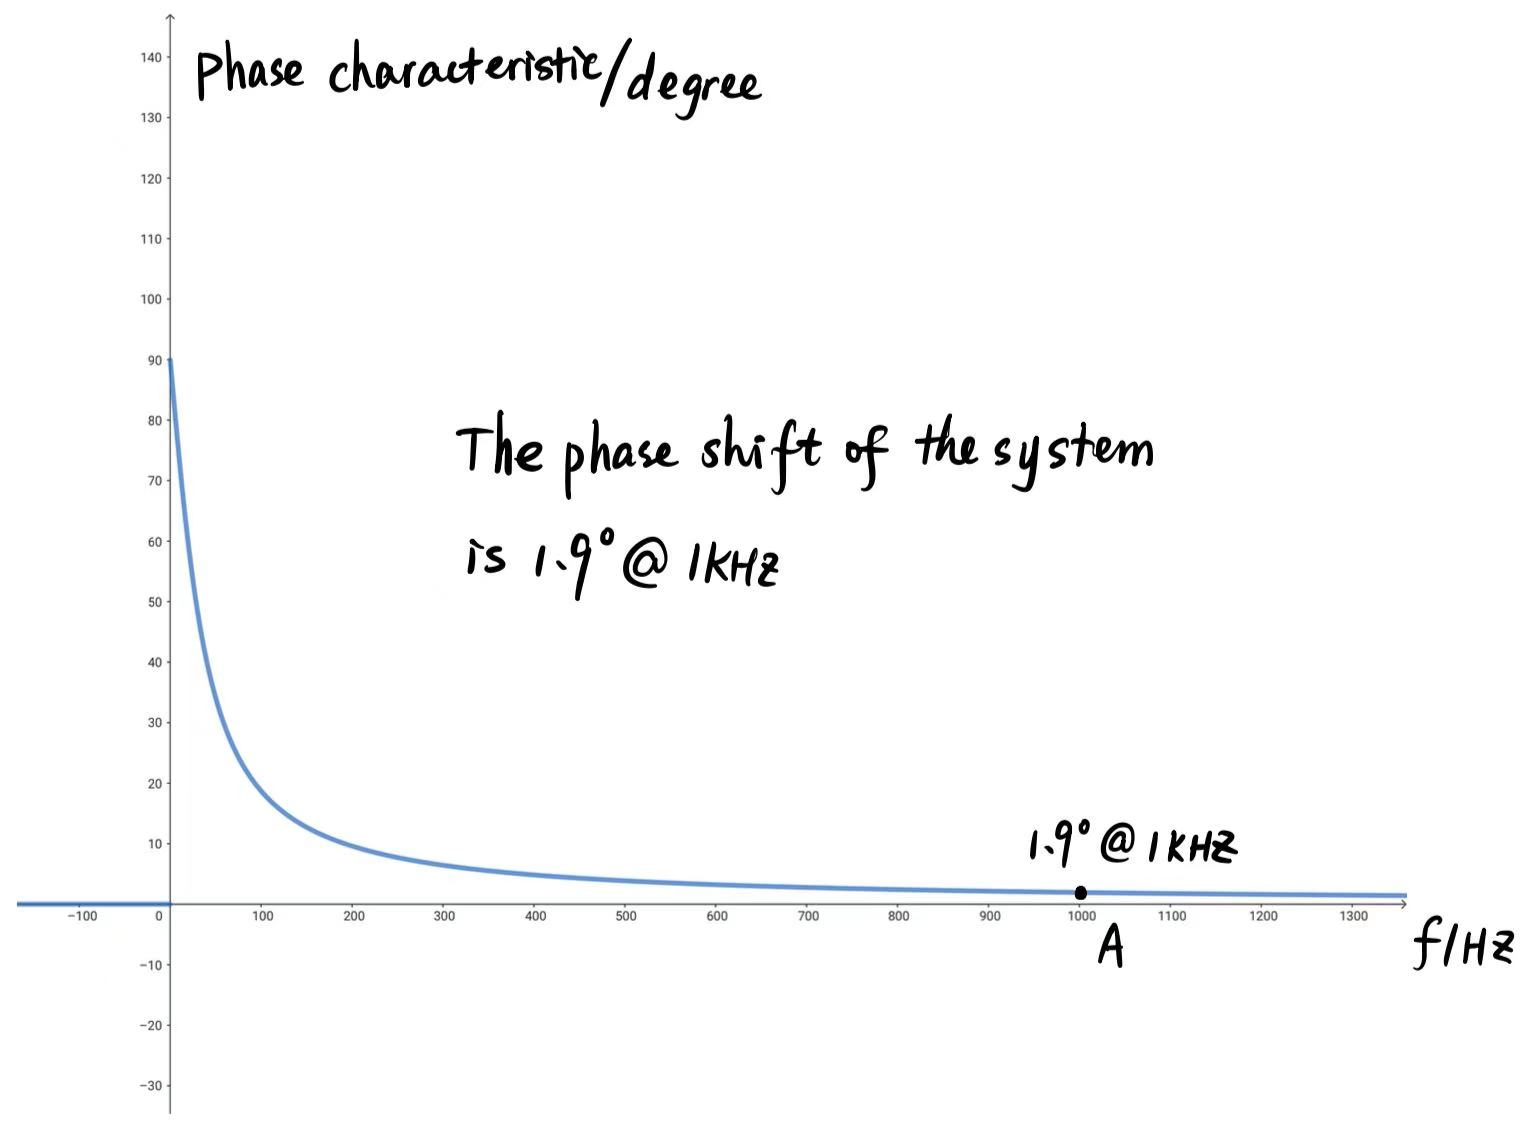
\includegraphics[width=0.7\textwidth]{ET2_1_analysis_outcome2.jpg}
		\caption{The analysis outcome of circuit (phase)}
		\label{fig:outcome2}
	\end{figure}
\end{enumerate}

% 讨论
\subsubsection{Discussion}
In this part, we will analyze and discuss the data we got in \cref{tab:tab1} and \cref{tab:tab2}, according to previous analysis.
\begin{enumerate}
	\item We visualized the experimental data and the results are shown below.
	
	\begin{figure}[htbp]
		\centering
		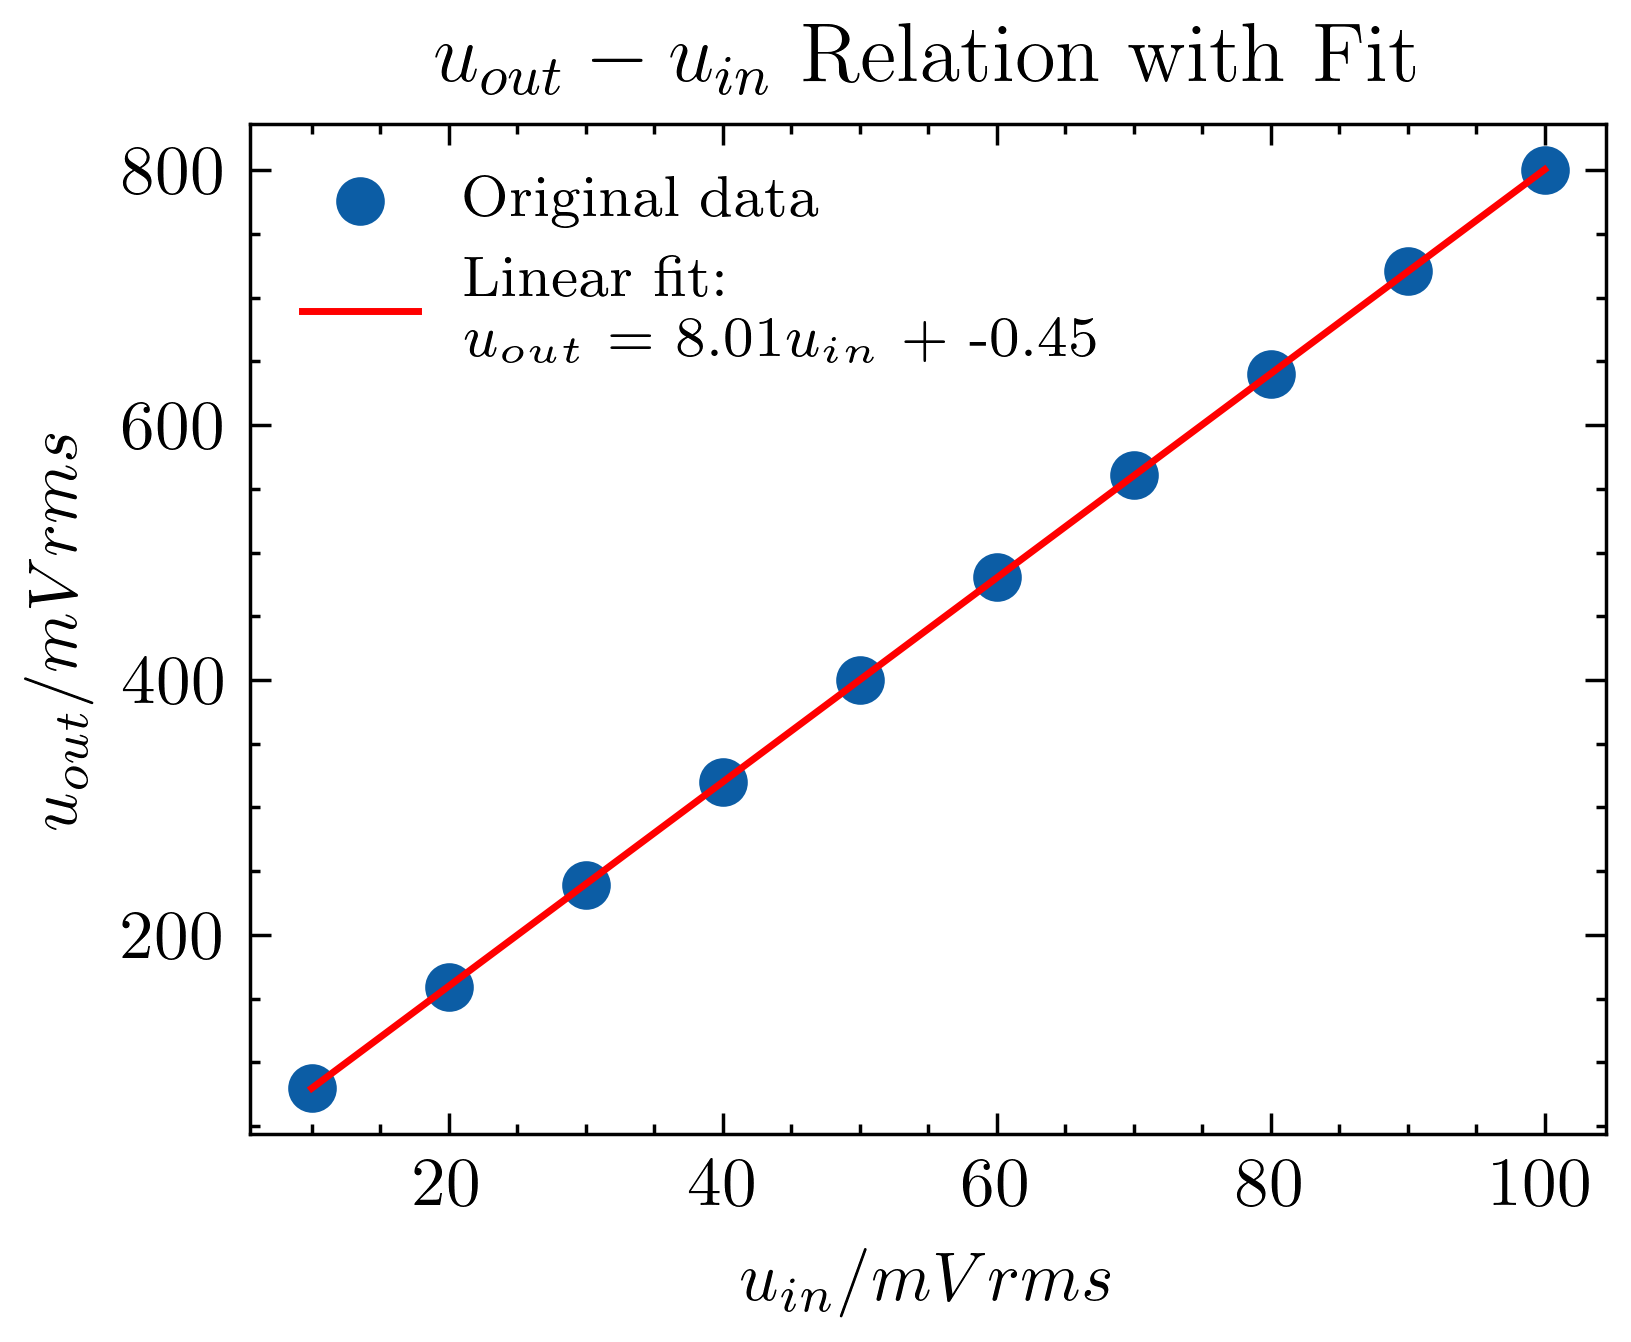
\includegraphics[width=0.7\textwidth]{ET2_1_dicussion1.png}
		\caption{Voltage gain vs. frequency}
		\label{fig:dicussion1}
	\end{figure}
	
	\begin{figure}[htbp]
		\centering
		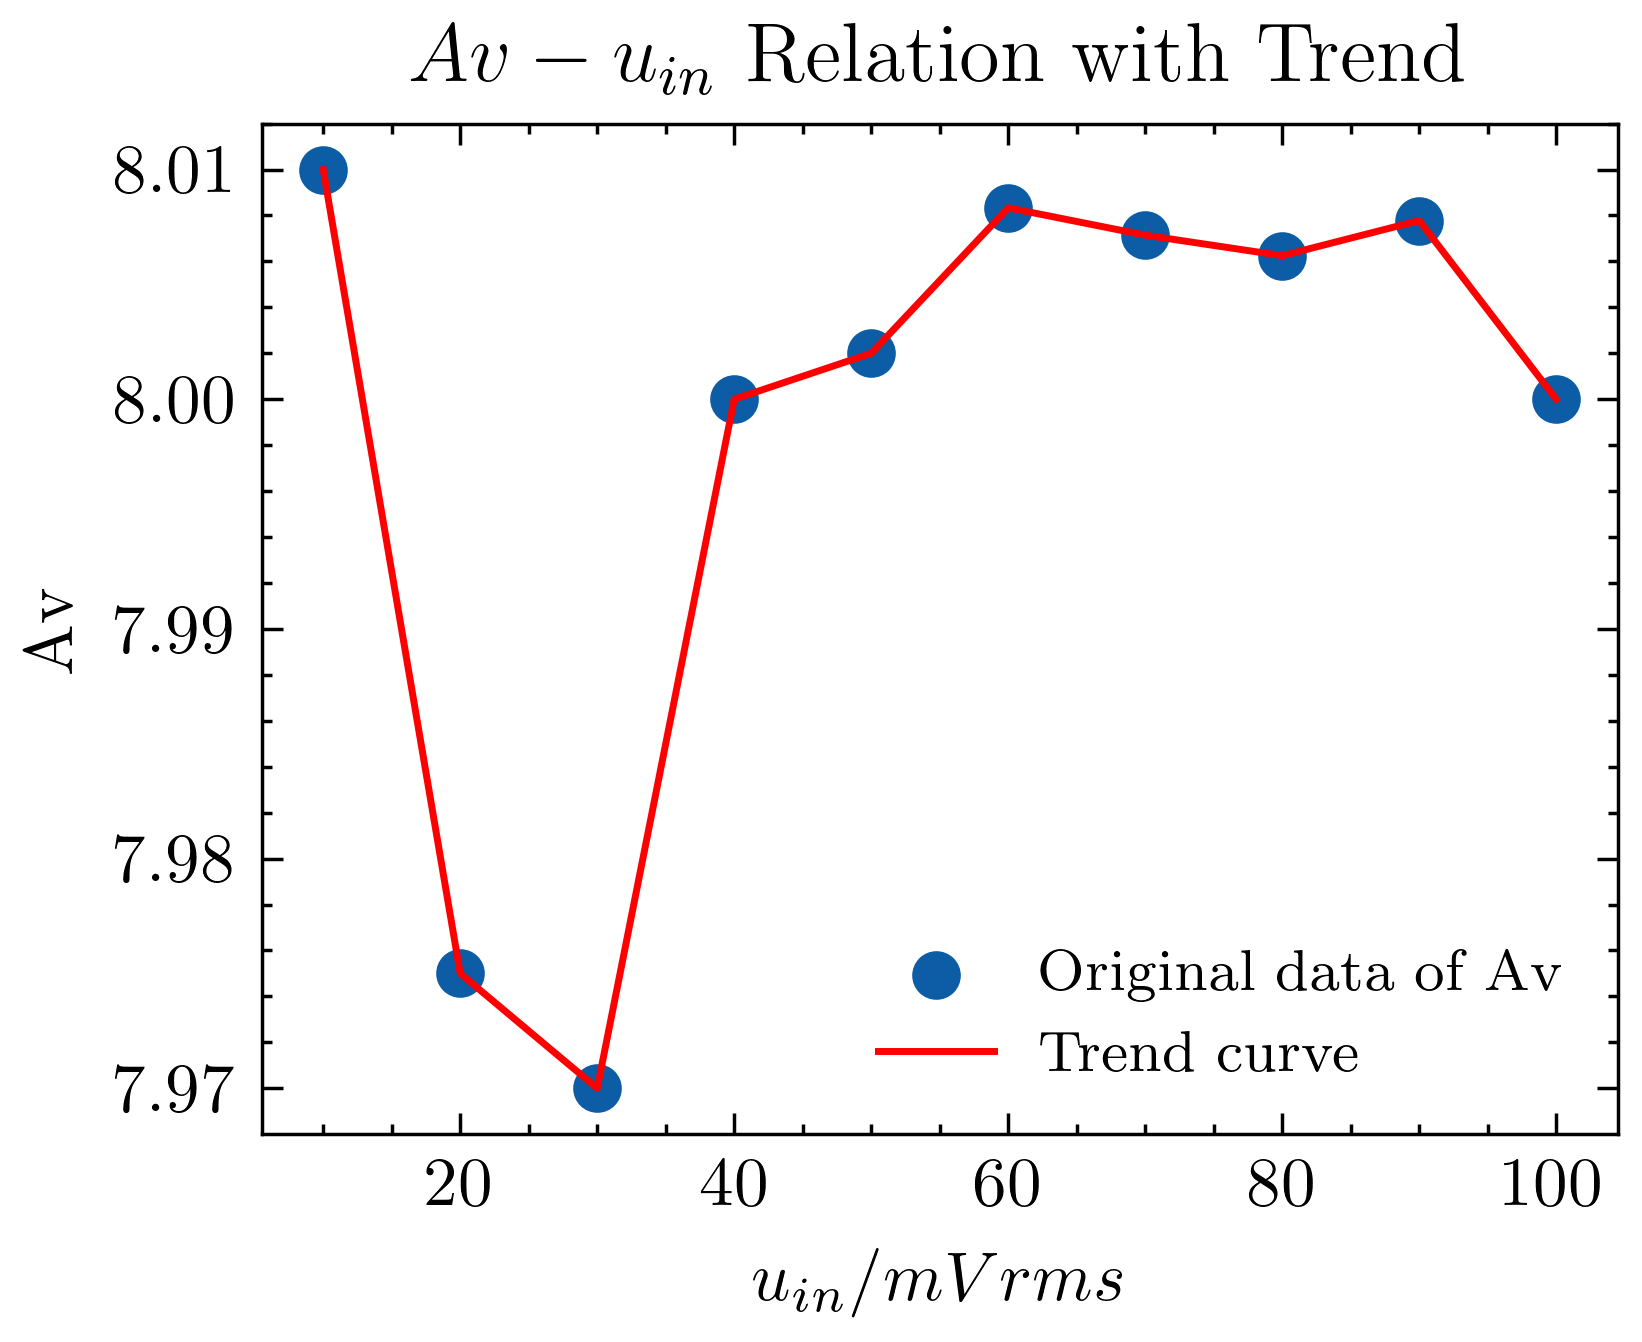
\includegraphics[width=0.7\textwidth]{ET2_1_dicussion2.png}
		\caption{Comparison of the experimentally determined voltage gain versus frequency relationship with the ideal case}
		\label{fig:dicussion2}
	\end{figure}
	
	\begin{figure}[htbp]
		\centering
		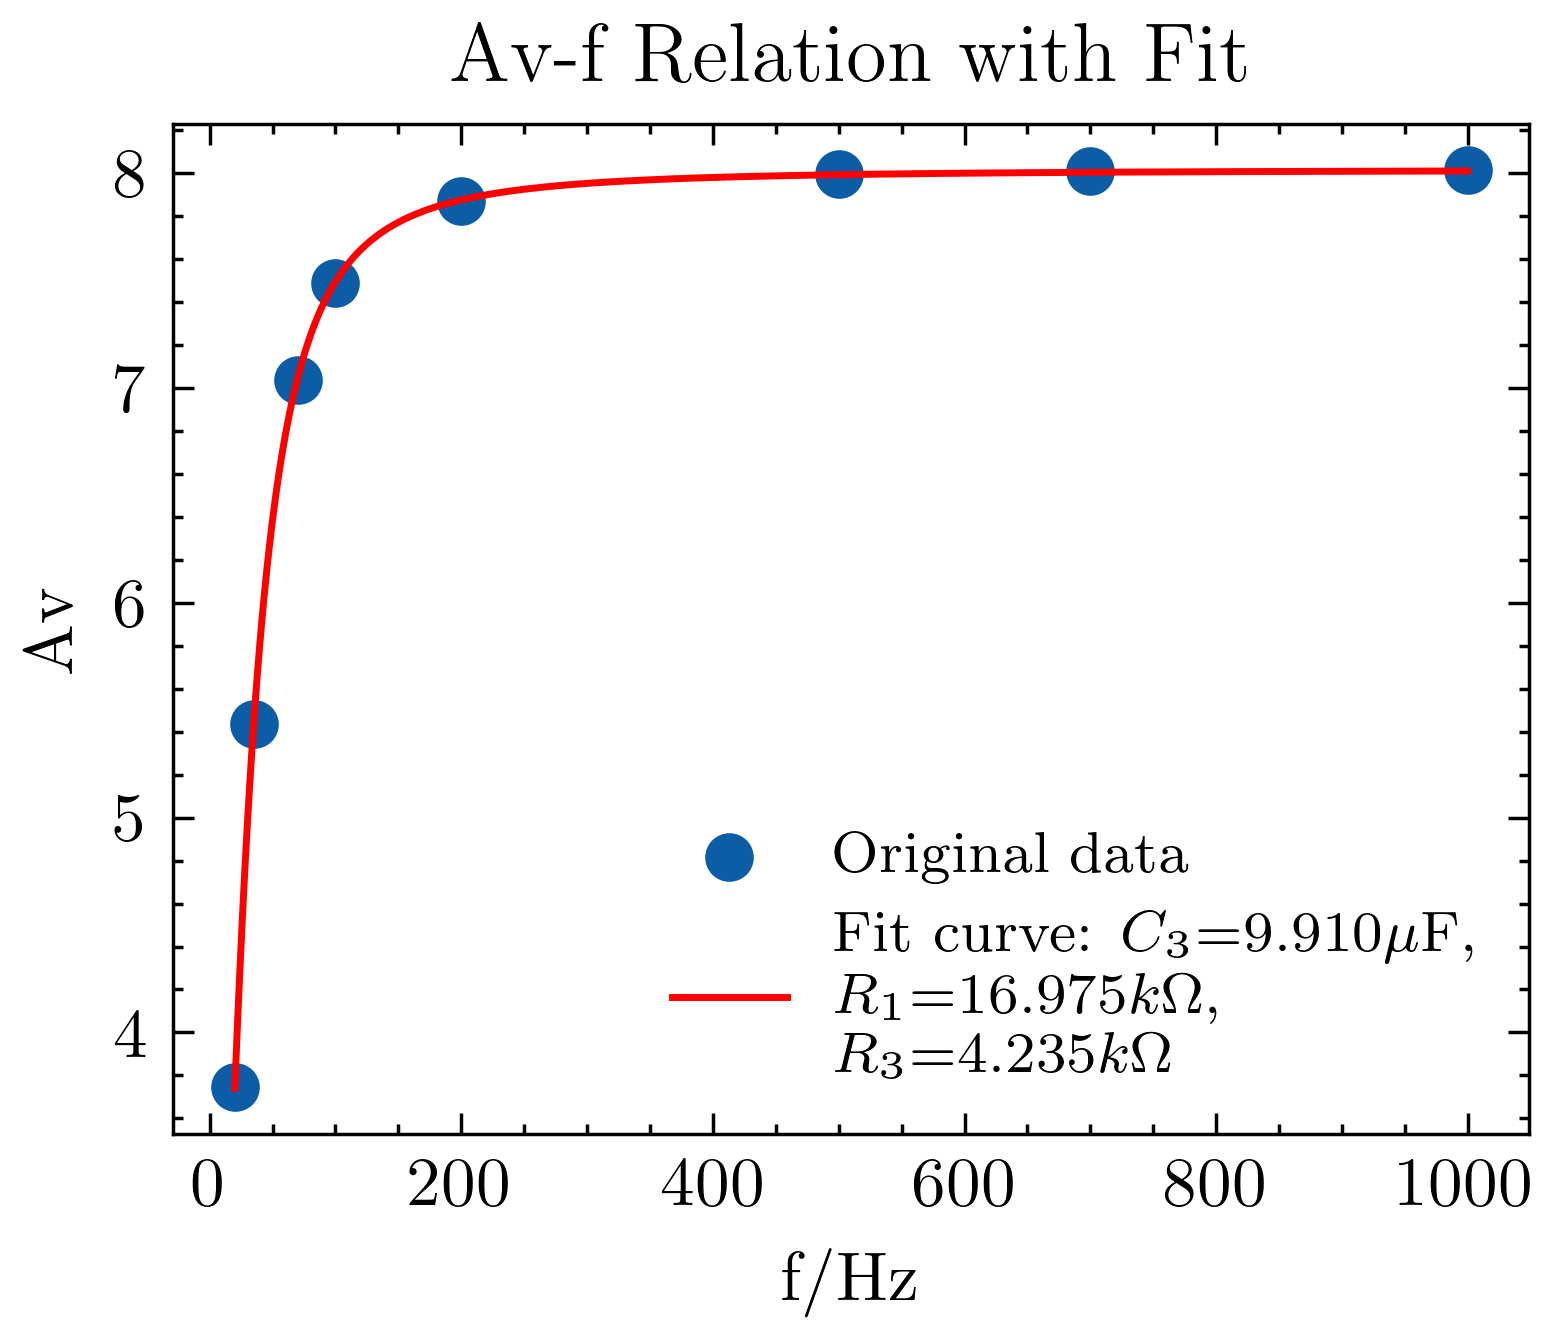
\includegraphics[width=0.7\textwidth]{ET2_1_dicussion3.png}
		\caption{Fitting of amplification factor (the relationship between output voltage and input voltage)}
		\label{fig:dicussion3}
	\end{figure}
	
	\begin{figure}[htbp]
		\centering
		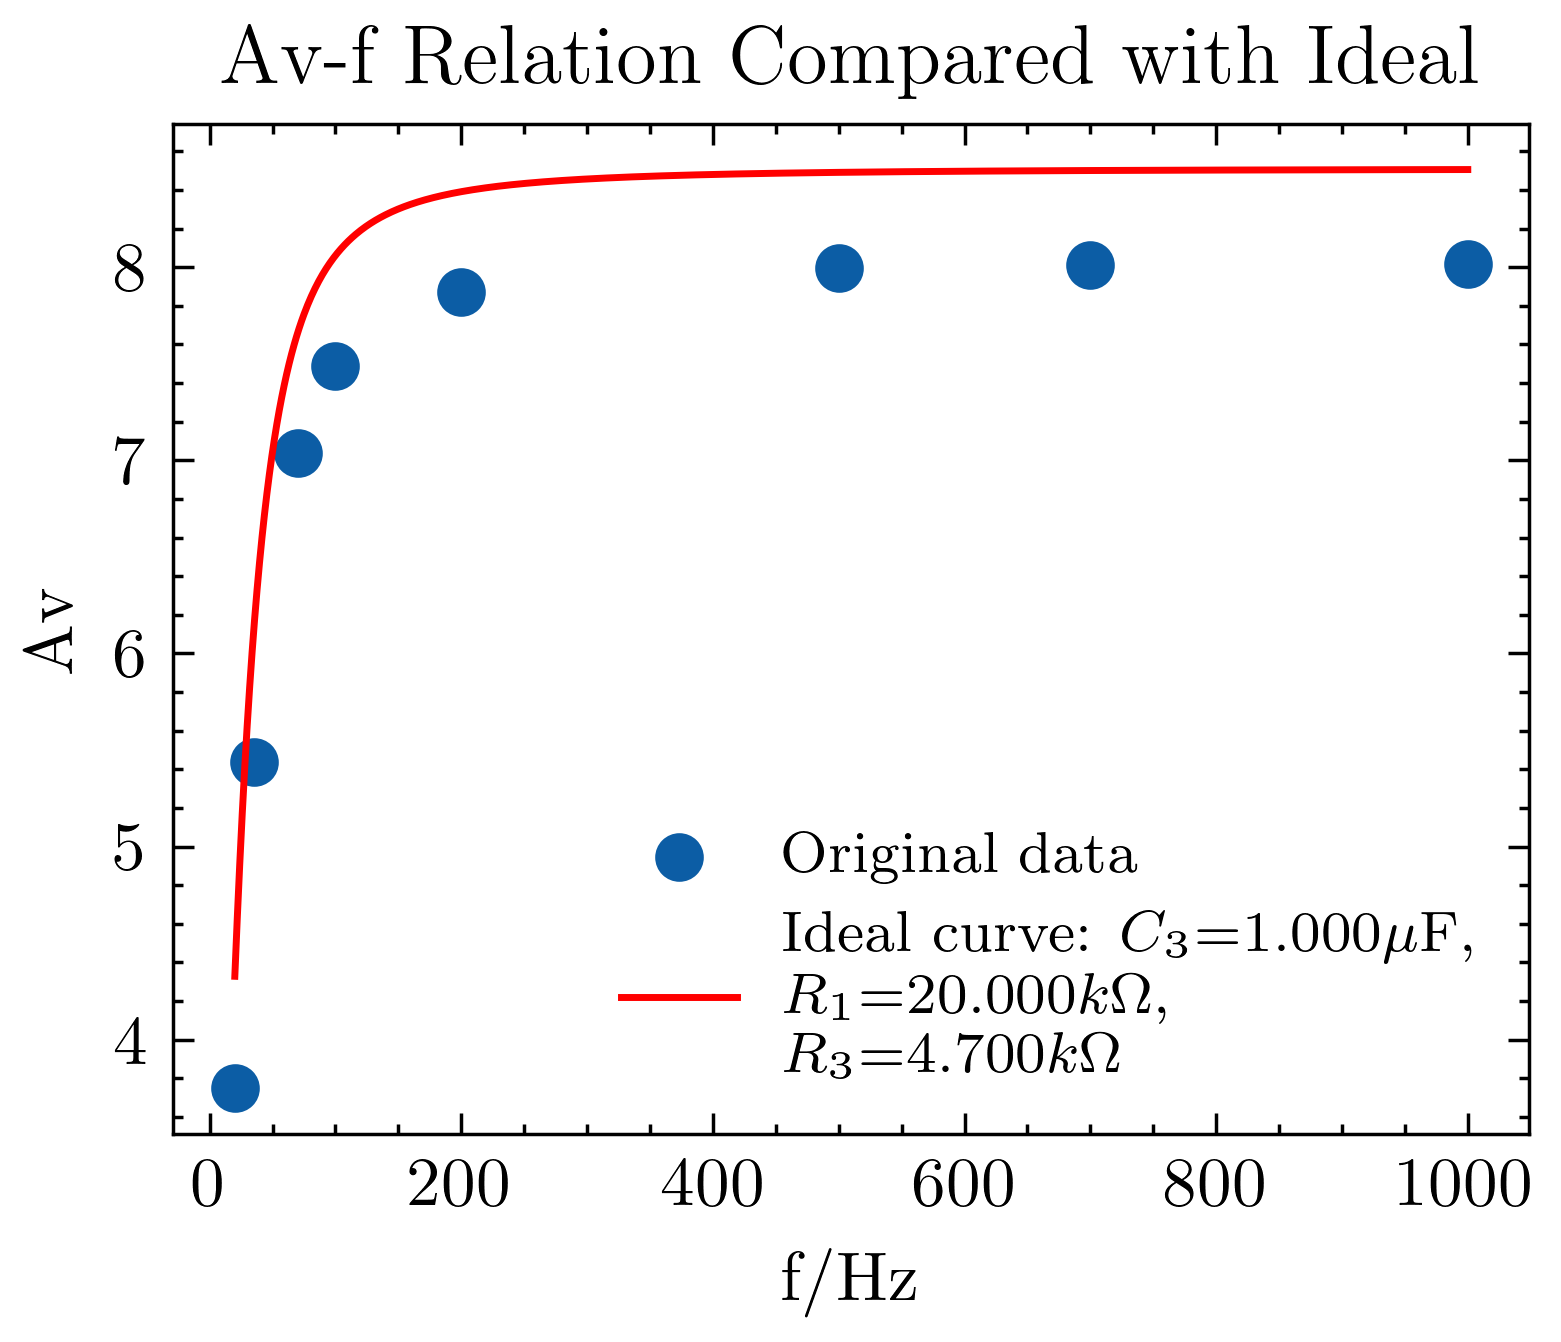
\includegraphics[width=0.7\textwidth]{ET2_1_dicussion4.png}
		\caption{Voltage gain variation trend with input voltage}
		\label{fig:dicussion4}
	\end{figure}
	
	\item What follows is a discussion of the above results.
	
	In \cref{fig:dicussion1}, we performed a linear fit on the experimental data. From the fitting parameters, we can see that the measured value of the voltage gain is 8.01, which is slightly different from the theoretical value of 8.51 we calculated, which is also reflected in \cref{fig:dicussion4}. On the other hand, we can see from \cref{fig:dicussion2} that the voltage gain changes randomly with the output voltage and there is no obvious functional relationship, which shows that our measurement still has a certain degree of reliability.
	
	In \cref{fig:dicussion3}, we visualize the relationship between the voltage gain and the frequency. It is worth noting that, as shown in the previous theoretical analysis, -3dB is right around 35Hz. In addition, we performed a fitting, and the figure shows that the values ​​of the components obtained by the fitting are somewhat different from the actual values.
	
	In \cref{fig:dicussion4}, we compare our measured results with our calculated theoretical predictions. Overall, the measured results are smaller. Especially in the low-frequency region, the measured voltage gain is significantly lower than the theoretically calculated value. The following are possible reasons and analysis for this difference:
	\begin{itemize}
		\item Capacitor deviation and ESR (equivalent series resistance)
		
		The theoretical curve is calculated based on ideal components, but in reality, capacitors will have manufacturing deviations and additional characteristics. For example, C3 (1.000 $\mu F$) in the figure may have a certain deviation and is not exactly 1 $\mu F$. In addition, the equivalent series resistance (ESR) of the capacitor will introduce additional losses, especially in the low-frequency band. These factors may affect the efficiency of the signal passing through the capacitor, resulting in reduced gain.
		
		\item Low-frequency impact of input coupling capacitor
		
		Amplifier circuits usually use coupling capacitors to isolate DC bias. These coupling capacitors have limited transmission capabilities for low-frequency signals. When the frequency is low, the impedance of the capacitor is large, which will limit the passage of the signal, resulting in signal attenuation and reduced gain. Therefore, at low frequencies, the actual measured gain may be lower than the theoretical value.
		
		\item Gain-bandwidth limitation of amplifier
		
		The gain-bandwidth product of LM4863 may be limited at low frequencies. Actual operational amplifiers usually have gain-bandwidth limitations in design. When the frequency is low, the gain is affected by the internal circuit characteristics of the amplifier, such as open-loop gain characteristics and frequency compensation. This may cause the gain in the low frequency band to be not as high as ideal.
		
		\item The influence of parasitic capacitance and wiring
		
		In actual circuits, parasitic capacitance and wiring inductance affect the frequency response of the amplifier circuit. Especially at low frequencies, the parasitic capacitance of the wiring may introduce phase shift and signal loss, resulting in low actual gain. In addition, the parasitic impedance present in the PCB wiring may interact with other components, thereby affecting the overall frequency response.
		
		\item Component accuracy in negative feedback network
		
		The theoretical gain in the figure is calculated based on the precise values ​​of R1 and R3. However, in actual circuits, the accuracy of these resistors (usually 5\% or 1\%) may have some deviation. Any slight deviation in the resistance value will change the proportion of negative feedback, resulting in the actual gain not being completely consistent with the theoretical calculated value, which may be more obvious at low frequencies.
		
		\item Temperature and power supply stability
		
		The performance of the amplifier circuit will also be affected by temperature changes, especially at low frequencies. The internal characteristics of the LM4863 are sensitive to temperature changes, which will affect the internal gain characteristics of the device, resulting in differences between the measured value and the theoretical value. In addition, the instability of the power supply voltage (ripple and noise) may also affect the gain at low frequencies.
		
		\item Test instrument and measurement error
		
		When measuring at low frequencies, the characteristics of the instrument itself may also affect the measurement results. For example, the low-frequency response of the signal source, the probe impedance of the oscilloscope, or the influence of the connecting line will cause certain errors in the measurement accuracy. These errors may not be obvious at high frequencies, but may be more prominent at low frequencies, resulting in deviations between the measured value and the theoretical value.
		
		\item Frequency response of coupling and decoupling capacitors
		
		The coupling capacitors (such as C4, C5) and decoupling capacitors (such as C1, C2) in the figure may also fail to fully function in the low frequency band. For example, the decoupling capacitors cannot fully eliminate low-frequency noise, which may affect the low-frequency gain of the amplifier. If the coupling capacitor is too small, it will have a great impact on the transmission of low-frequency signals, thereby reducing the low-frequency gain.
	\end{itemize}
	
\end{enumerate}

% 总结
\subsubsection{Conclusion}

The performance of the LM4863 amplifier circuit is analyzed by welding the Bluetooth speaker. The actual operation of the circuit is evaluated by measuring the voltage gain and power gain, and the factors affecting the low frequency performance are discussed.

\begin{itemize}
	\item The experimental results show that the voltage gain of LM4863 amplifier circuit varies with frequency and reaches the -3dB point around 35Hz, which is consistent with the theoretical analysis.
	\item However, the experimentally measured voltage gain value is usually lower than the theoretically calculated value, especially in the low frequency region. The measured voltage gain is 8.01, slightly lower than the theoretical value of 8.51. The power gain is about 17.0, or 12.3 dB@1kHz. 
	\item These results suggest that the performance of a circuit at low frequencies may be affected by a variety of factors, including capacitor bias, input coupling capacitor influence, amplifier gain-bandwidth limitations, parasitic capacitance and wiring influence, component accuracy in a negative feedback network, temperature and power supply stability, test instruments and measurement errors, and the frequency response of coupling and decoupling capacitors.
\end{itemize}
